\documentclass[12pt,fleqn]{article}\usepackage{../../common}
\begin{document}
Sonlu Öğeler Metotu (Finite Elements Method -FEM-) - 3

İki boyutta FEM kullanımına gelelim. Diyelim ki alttaki gibi bir problem
yarattım,

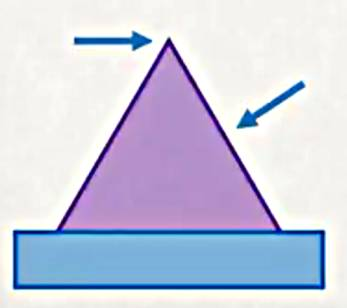
\includegraphics[width=10em]{compscieng_bpp45fem3_01.jpg}

Üçgen şeklinde bir yapı var, onun üzerinde iki noktadan kuvvet uygulanmış, şimdi
bu üçgendeki stres ve gerilmeyi bulmak istiyorum. Bu problemi nasıl çözerdik?
Euler-Bernoulli kiriş denklemini kullanmak zor, şekil ona uygun değil. Zor bir
iş.

Fakat üstteki problemi bir FEM problemine dönüştürürsem işler
kolaylaşabilir. Bir ızgara oluşturabilirim mesela,

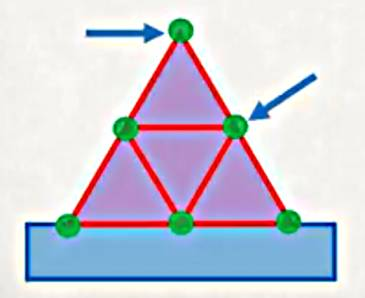
\includegraphics[width=10em]{compscieng_bpp45fem3_02.jpg}

Altı tane düğüm noktası ortaya çıktı, düğümsel yer değişimini hesaplayabiliriz,
ve dikkat edersek düğümlerin üçü altta sabitlenmiş halde. Ama hesapla devam
etmem için o görülen tüm yapının direngenliğini (stiffness) bulmam lazım, bu
derste göreceğimiz ilk konu o ızgaradaki her üçgenin ayrı ayrı direngenliğini
bulabilmek çünkü düğümler üzerindeki kuvvetleri biliyorsam (ki biliyorum)
direngenliği kullanarak çözümde ilerleyebilirim.

Hatırlarsak çubuk ve kirişleri modellerken bir yaklaşıklama fonksiyonu
kullanmıştım, bu fonksiyon yukarı ya da yana doğru bir hareketi yaklaşık temsil
ediyordu. İki boyutta benzer bir prosedürü kullanacağız, fakat tek yön yerine
iki yönü aynı anda temsil etmemiz gerekecek.

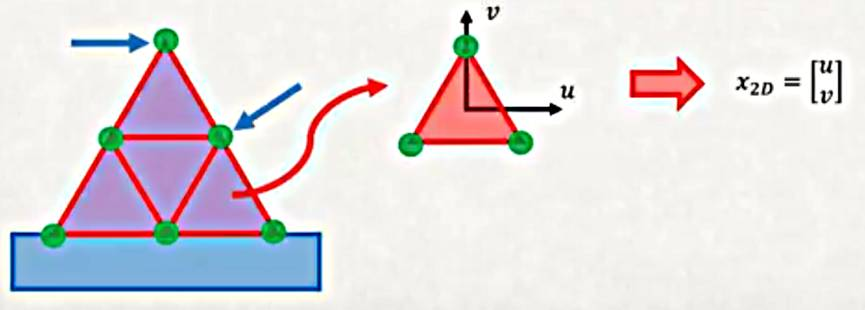
\includegraphics[width=20em]{compscieng_bpp45fem3_03.jpg}






















[devam edecek]

Kaynaklar

[1] Petitt, {\em Intro to the Finite Element Method}, University of Alberta,
    \url{https://www.youtube.com/watch?v=2iUnfPRk6Ro&list=PLLSzlda_AXa3yQEJAb5JcmsVDy9i9K_fi}

[2] Petitt, {\em Finite Element Method Theory}, University of Alberta,
    \url{https://www.youtube.com/watch?v=2iUnfPRk6Ro&list=PLLSzlda_AXa3yQEJAb5JcmsVDy9i9K_fi}

\end{document}
